\section{图形渲染技术}

\subsection{OpenGL图形库}

\par OpenGL(Open Graphics Library)是一个由美国硅图技术公司开发,现由Khronos Group维护的跨语言、跨平台的专业图形库,被广泛应用于计算机辅助设计(Computer Aided Design,CAD)、虚拟现实、科学可视化、游戏引擎和飞机模拟等领域。

\par OpenGL的设计基于一个状态机,其内部定义了近300个用于绘制不同场景的函数,其中的大部分函数用于更改内部状态,而不是直接操作图形数据。
它支持多种渲染技术,包括纹理映射、阴影生成、抗锯齿、透明度、光照模型等。

\par OpenGL主要特点是跨平台性和扩展性,可以运行在各种操作系统(如Windows、Mac OS、Linux等)和硬件平台上。由于OpenGL是一个开放标准,因此可以被各种硬件制造商和开发者自由地使用和扩展。

\par 此外,OpenGL的另一个显著特点是强大的性能,随着GPU等计算机图形硬件的不断发展,可以更高效地渲染复杂的三维场景,以及支持新的渲染技术和效果。

\subsection{渲染管线}
\par 图形渲染管线\cite{OpenGL_graphics_system}是硬件和软件之间的抽象,输入需要渲染的三维物体的相关描述信息(如顶点坐标、顶点颜色、顶点纹理等),
经过一系列变换与渲染的过程,在计算机屏幕输出二维图像。如图\ref{fig:glpipeline}所示,主要分为两个阶段:几何阶段和光栅化阶段。

\begin{figure}[htb]
	\centering
	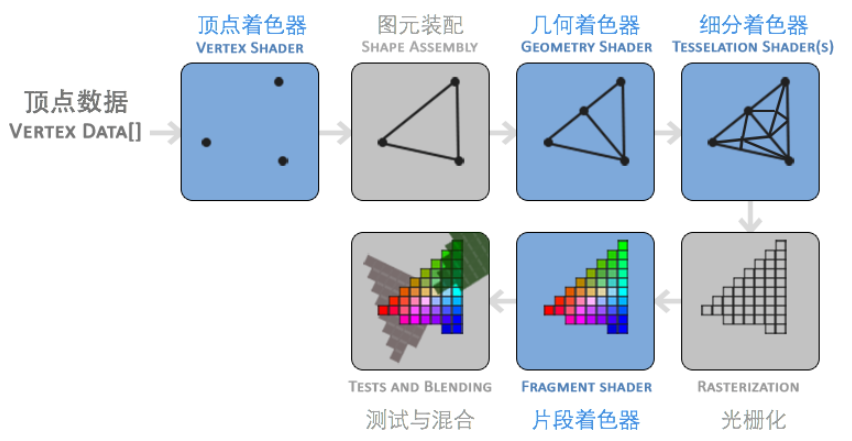
\includegraphics[width=0.9\textwidth]{figures/opengl_pipeline.png}
	\caption{OpenGL渲染管线}
	\label{fig:glpipeline}
	\note{注:OpenGL渲染管线的两个主要阶段:几何阶段和光栅化阶段。}
\end{figure}

\paragraph{几何阶段}

\par 该阶段负责处理所有关于几何图形(如顶点和线)的数据。主要包括以下步骤:

\subparagraph{顶点着色器(Vertex Shader)}
\par 这是GPU上运行的第一个程序,负责处理三维空间中的顶点数据。它的任务包括变换坐标,计算光照和颜色等。

\subparagraph{图元装配(Primitive Assembly)}
\par 顶点着色器处理完顶点数据后,将这些顶点组装成几何图元,如点、线、三角形等。

\subparagraph{几何着色器(Geometry Shader)}
\par 可选阶段,可以在此创建新的顶点或者丢弃某些几何图元。

\subparagraph{裁剪(Clipping)}
\par 丢弃不会出现在最终屏幕上的几何图元。

\paragraph{光栅化阶段}
\par 该阶段负责将几何图形转换为像素图像,主要包括以下步骤:

\subparagraph{光栅化(Rasterization)}
\par 将裁剪后的几何图形转换为像素图像,得到的结果称为片元(Fragment)。

\subparagraph{片元着色器(Fragment Shader)}
\par 将每个片元通过片元着色器进行处理,计算最终的颜色和其他属性。

\subparagraph{Alpha测试和混合(Alpha Testing and Blending)}
\par 最后,检查每个片元的透明度并混合在一起,得到最终的像素颜色。